%%%%%%%%%%%%%%%%%%%%%%%%%%%%%%%%%%%%%%%%%
% Diaz Essay
% LaTeX Template
% Version 2.0 (13/1/19)
%
% This template originates from:
% http://www.LaTeXTemplates.com
%
% Authors:
% Vel (vel@LaTeXTemplates.com)
% Nicolas Diaz (nsdiaz@uc.cl)
%
% License:
% CC BY-NC-SA 3.0 (http://creativecommons.org/licenses/by-nc-sa/3.0/)
%
%%%%%%%%%%%%%%%%%%%%%%%%%%%%%%%%%%%%%%%%%

%----------------------------------------------------------------------------------------
%	PACKAGES AND OTHER DOCUMENT CONFIGURATIONS
%----------------------------------------------------------------------------------------

\documentclass[11pt]{diazessay} % Font size (can be 10pt, 11pt or 12pt)

%----------------------------------------------------------------------------------------
%	TITLE SECTION
%----------------------------------------------------------------------------------------

\title{\textbf{Minarea regulilor de asociere} \\ 
{\Large\itshape  Algoritmul Apriori}} % Title and subtitle

\author{\textbf{Stîngă Alexandra}} 

\usepackage{listings}
\usepackage{color}

\definecolor{dkgreen}{rgb}{0,0.6,0}
\definecolor{gray}{rgb}{0.5,0.5,0.5}
\definecolor{mauve}{rgb}{0.58,0,0.82}

\lstset{frame=tb,
  language=Java,
  aboveskip=3mm,
  belowskip=3mm,
  showstringspaces=false,
  columns=flexible,
  basicstyle={\small\ttfamily},
  numbers=none,
  numberstyle=\tiny\color{gray},
  keywordstyle=\color{blue},
  commentstyle=\color{dkgreen},
  stringstyle=\color{mauve},
  breaklines=true,
  breakatwhitespace=true,
  tabsize=3
}

%----------------------------------------------------------------------------------------

\begin{document}

\maketitle % Print the title section

%----------------------------------------------------------------------------------------
%	ABSTRACT AND KEYWORDS
%----------------------------------------------------------------------------------------

%----------------------------------------------------------------------------------------
%	ESSAY BODY
%----------------------------------------------------------------------------------------

\section*{Introducere}

Data mining este procesul de descoperire a patternurilor în seturi de date de mari dimensiuni folosind modalități de machine learning, statistică și baze de date. Data mining, mineritul de date în traducere liberă, are rolul de a extrage în mod inteligent informația dintr-un set de date și să o transforme într-o structură ulterior folosită în luarea deciziilor.

Un algoritm clasic de data mining este algoritmul Apriori. Acesta a fost propus de Agrawal și Srikant in 1994 și este folosit pentru minarea itemseturilor frecvente și generarea regulilor de asociere.
%------------------------------------------------

\section*{Reguli de asociere. Exemplu}

Algoritmul apriori este folosit în găsirea itemseturilor frecvente într-o bază de date pentru reguli de asociere booleene. Numele algoritmului este Apriori deoarece se folosește de cunoaște dinainte proprietățile itemseturilor.

Acest algoritm constă într-o căutare iterativă în care k-itemseturile frecvente sunt folosite pentru a găsi (k+1)-itemseturile frecvente.Algoritmul începe prin determinarea 1-itemseturilor frecvente.Pentru aceasta se scanează baza de date și se determină suportul(numărul de apariții) fiecarui element din BD,care se va compara cu suportul minim. Itemseturile alese vor fi cele din care se vor genera 2-itemseturile, tot așa până când mulțimea generală k-itemset este vidă.

\begin{figure}[h]
	\centering
	\caption{Schema logică a algoritmului Apriori}
	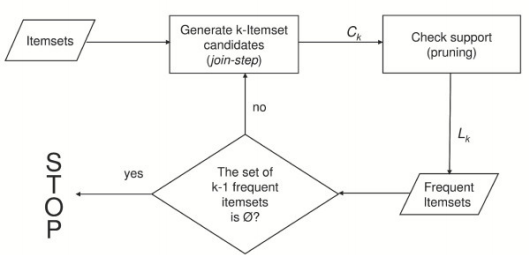
\includegraphics[scale=0.40]{apriori.png}   	
\end{figure}

Pentru a mări eficiența generării itemseturilor frecvente se folosesc următoarele proprietăți: toate subseturile unui itemset frecvent trebuie să fie frecvente și dacă un itemset este infrecvent atunci toate superseturile vor fi infrecvente.

În continuare este prezentat un exemplu practic folosind algoritmul descris mai sus. Datele de input sunt baza de date cu tranzacțiile dintr-un magazin, suportul minim care este 2 și confidența 4.

\begin{table}[h]
\caption{The dataset.}
\centering
\begin{tabular}{llll}
		\toprule
		\cmidrule(r){1-2}
		ID & Transaction \\
		\midrule
		1 & unt, oua, lapte &  \\
		2 & paine, unt &  \\
      	3& paine, oua, lapte &  \\
      	4& paine, unt, oua, lapte  &  \\
      	5& oua, lapte, salam  &  \\
      	6& paine, oua  & 
\end{tabular}
\end{table}

Calculăm  frecvența fiecărui itemset prin scanări repetate ale bazei de date.

\begin{table}[h]
\caption{The items and their frequence.}
\centering
\begin{tabular}{llll}
		\toprule
		\cmidrule(r){1-2}
		Itemset & Frequence \\
		\midrule
		unt & 3 &  \\
		oua & 5&  \\
      	lapte & 4 &  \\
      	paine& 4&  \\
      	salam & 1& 
\end{tabular}
\end{table}

Comparând frecvența fiecăruia cu suportul minim obținem 1-itemset.

\begin{table}[h]
\caption{The items and their frequence.}
\centering
\begin{tabular}{llll}
		\toprule
		\cmidrule(r){1-2}
		Itemset & Frequence \\
		\midrule
		unt & 3 &  \\
		oua & 5&  \\
      	lapte & 4 &  \\
      	paine& 4&  \\
\end{tabular}
\end{table}

Itemsetul de k = 2 valori este obținut prin unirea listei anterioare de itemseturi cu ea însuși. Condiția de unire este aceea ca cele 2 liste să aibă k-2 elemente în comun.

Se verifică dacă toate subseturile unui itemset sunt frecvente sau nu. În cazul în care itemsetul nu este frecvent va fi elliminat.
 
De exemplu subseturile itemsetului [unt, oua] sunt [unt] și [ouă] care sunt frecvente.

La fiecare pas se calculează suportul fiecărui itemset parcurgând baza de date. Dacă suportul itemsetului este mai mare decât suportul minim, atunci itemsetul va face parte din lista finală de itemseturi din care vor fi generate k+1 itemseturi.

\begin{table}[h]
\caption{The itemsets and their frequence.}
\centering
\begin{tabular}{llll}
		\toprule
		\cmidrule(r){1-2}
		Itemset & Frequence \\
		\midrule
		unt, oua & 2 &  \\
		unt, lapte & 2&  \\
      	unt, paine & 2 &  \\
      	oua, lapte & 4&  \\
      	oua, paine & 3&  \\
      	lapte, paine & 2&  \\
\end{tabular}
\end{table}

Itemsetul de 3 valori este:

\begin{table}[h]
\caption{The itemsets and their frequence.}
\centering
\begin{tabular}{llll}
		\toprule
		\cmidrule(r){1-2}
		Itemset & Frequence \\
		\midrule
		unt, oua, lapte & 2 &  \\
      	oua, paine, paine & 2 &  \\
\end{tabular}
\end{table}

Aici algoritmul se oprește deoarece nu se mai pot genera itemseturi de lungime 4. După ce s-au descoperit toate itemseturile frecvente, se trece la generarea regulilor de asociere. Pentru asta este nevoie de calcularea confidenței fiecărei reguli.\\

O regulă de asociere arată în felul următor: 
\begin{equation}
Confidence(A->B)=SupportCount(A\cup B)/SupportCount(A)
\end{equation}

Itemsetul [unt, oua, lapte] are următoarele reguli de asociere:\break
[unt -> ouă] => lapte <=> support(unt,ouă, lapte)/support(unt,ouă) = 2/2 = 100 \break
[unt -> lapte] => ouă <=> support(unt,ouă, lapte)/support(unt,lapte) = 2/2 = 100 \break
[ouă -> lapte] => unt <=> support(unt,ouă, lapte)/support(ouă,lapte) = 2/4 = 50 \break
[unt] -> [ouă -> lapte] <=> support(unt,ouă, lapte)/support(unt) = 2/3 = 66 \break
[ouă] -> [unt -> lapte] <=> support(unt,ouă, lapte)/support(ouă) = 2/5 = 40 \break
[lapte] -> [unt -> ouă] <=>  support(unt,ouă, lapte)/support(lapte) = 2/4 = 50 \break

%------------------------------------------------

\section*{Algoritmul apriori. Cod}

Aplicația practică se folosește de baza de date din primul tabel și generează regulile de asociere corespunzătoare.

Baza de date este încărcată în memorie, într-o structură de date de tip listă de Stringuri, pentru folosiri ulterioare.

\begin{lstlisting}
//read database
private ArrayList<String> readDB() {
		
	  ArrayList<String> tranzactions = new ArrayList<>();
	  BufferedReader br = null;
	  String st = null; 
	  
	try {
		br = new BufferedReader(new FileReader(file));
	} catch (FileNotFoundException e1) {
		// TODO Auto-generated catch block
		e1.printStackTrace();
	} 
	  
	 try {
		while ((st = br.readLine()) != null) {
			tranzactions.add(st);
			nrTranzactii++;
			}
		} catch (IOException e) {
			// TODO Auto-generated catch block
			e.printStackTrace();
		} 

		return tranzactions;
	}
\end{lstlisting}

În primul pas al algoritmului se determină itemseturile frecvente de k=1. Se parcurge lista de tranzacții si se stochează suportul fiecărui item în tabela newCandidates. După terminarea acestui pas se aleg itemurile care depășesc suportul minim și se trece la generarea itemseturilor de k+1.

\begin{lstlisting}
//generate itemset of size 1
private ArrayList<String> itemsetSize1(ArrayList<String> candidates){
		
		LinkedHashMap<String, Integer> newCandidates = new LinkedHashMap<>();
		ArrayList<String> itemsList = new ArrayList<>();	
		
		Iterator<String> li = tranzactions.iterator();
		String tmpString;
		List<String> trans_items;
		
		//init the candidates hashmap
		int count = 0;
		candidates.forEach(candidat -> newCandidates.put(candidat, count));
//		candidates.forEach(i -> System.out.println(i));
		
		while(li.hasNext()) {
			//for each transaction
			tmpString = li.next();
			trans_items =  Arrays.asList(tmpString.split(",[ ]*"));
			
			//update the counter of each item
			for(int i = 0; i<trans_items.size(); i++) {
				newCandidates.put(trans_items.get(i), newCandidates.get(trans_items.get(i)) + 1);
			}		
		}
		
		//check if the frecquence of each item > minim_support
		for (Entry<String, Integer> m: newCandidates.entrySet()) { 
			if(m.getValue() >= minSup )
				itemsList.add(m.getKey());
        } 
		
		//Sysout chosen items
		for (Entry<String, Integer> m: newCandidates.entrySet()) { 
			System.out.println(m.getKey()+" "+m.getValue()); 
		} 
		
		return itemsList;
	}
\end{lstlisting}

După ce s-a determinat suportul fiecărui produs, se poate trece la generarea itemseturilor de 2,3,... etc.

\begin{lstlisting}
//generate itemset of size N
private ArrayList<ArrayList<String>> generateNitems(ArrayList<ArrayList<String>> items, int cicle){
		
		System.out.println("Cicle "+cicle);
		ArrayList<ArrayList<String>> newItems = new ArrayList<>();
		ArrayList<String> tmpSet1,tmpSet2, tmpItem = new ArrayList<>();
		
		int i,j;
		for(i = 0; i < items.size(); i++) {
			for(j = i+1;j < items.size(); j++) {
				
				/*get the 2 list*/
				tmpSet1 = items.get(i);
				tmpSet2 = items.get(j);
				
				/*det if are cicle-1 elem common*/
				if(canJoin(tmpSet1, tmpSet2,cicle)) {
					tmpItem = joinList(tmpSet1, tmpSet2);
					
					/*det if has frequent subsets*/
					if(hasFrequent(items,tmpItem,cicle))
						newItems.add(tmpItem);
				}
			}
		}
		
//		System.out.println("generateNitems "+newItems.toString());
		return newItems;
	}
\end{lstlisting}

Generarea regulilor de asociere se face după formula prezentată mai sus.

\begin{lstlisting}
//assoc rules
private void generateAssocRules(ArrayList<ArrayList<String>> assocCandidates) {
	
		System.out.println("Association rules");
		assocCandidates.forEach(i -> System.out.println(i));
		int pairCount;
		
		LinkedHashMap<String, Integer> onesHashMap = new LinkedHashMap<>();
		for(int i=0;i<assocCandidates.size();i++) {
			assocCandidates.get(i).forEach(candidat -> onesHashMap.put(candidat, 0));
		}
		
		//count itemset appearences
		countOne(onesHashMap);
		
		if(assocCandidates.get(0).size() == 2) {
			for(int index =0;index < assocCandidates.size(); index++) {
				pairCount = countPair(assocCandidates.get(index));
				associationsHashMap.put(assocCandidates.get(index), ((float) pairCount/onesHashMap.get(assocCandidates.get(index).get(0))));
			}
		}
		
		//Sysout the confidence of every rule
		for (Entry<ArrayList<String>, Float> m: associationsHashMap.entrySet()) { 
			System.out.println(m.getKey()+" "+m.getValue()); 
		} 
	
	}
\end{lstlisting}

%----------------------------------------------------------------------------------------
%	BIBLIOGRAPHY
%----------------------------------------------------------------------------------------

\bibliographystyle{unsrt}

\bibliography{sample.bib}

%----------------------------------------------------------------------------------------

\end{document}
